% Chapter 2

\chapter{Renormalization and QED Radiative Corrections} % Chapter title

\label{ch:Renorm} % For referencing the chapter elsewhere, use \autoref{ch:name}

%----------------------------------------------------------------------------------------

\section{Divergences, regularization and renormalization in QED}

When calculating loop Feynman diagrams in QED at some point the integrals will diverge. To cure these divergences we have to go through the process of renormalization. Renormalization is a formal manipulation, embedded inside the quantum field theory formalism, which allows us to calculate finite testable expectation values and scattering amplitudes. However we do not know how physics decribes high energy processes : there may be high energy virtual particles contributing to the loop diagrams and they would definitely impact the divergence of the integral. Thus we could say that renormalization is a procedure allowing to calculate reasonably the effects of the low-energy physics independently to what happens at high energies.

To describe the renormalization process, consider the electron self-energy. Defining the full electron propagator $G_F(p)$ by including order-by-order in the perturbation theory the corrections to the Feynman-Green function \cite{ItzyksonZuber} :
%
\begin{equation}
    \begin{split}
      G_F(p) =
      \feynmandiagram [layered layout, horizontal=d to b] {
  b -- [anti fermion] d, };
  +
  \feynmandiagram [layered layout, horizontal=a to b]{
  a -- [anti fermion] b
  -- [anti fermion] c
  -- [anti fermion] d,
  b -- [photon, half left, looseness=1.5] c,};
  +
  \mathscr{O}(e^4_0) \\
      = \frac{i}{\slashed{p}-m_0+i\epsilon} + G^{(1)}_F(p) + \mathscr{O}(e^4_0)
    \end{split}
\end{equation}
%
where $e_0$ and $m_0$ are the \textit{bare} charge and mass parameters and $G^{(1)}_F(p)$ is a divergent term. The renormalization procedure then follows three steps :

\begin{enumerate}
  \item \textbf{Regularization} : set a new \textit{finite} integral $G^{(1)}_F(p,\Lambda)$ with a dependence with the \textit{cut-off scale}\footnote{A cut-off is often introduced in text books to explain the procedure. However, all modern practical calculations are performed with \textit{dimensional regularization}.} $\Lambda$ yielding :
  \begin{equation}
    G^{(1)}_F(p,\Lambda) \xrightarrow{\Lambda\rightarrow\infty} G^{(1)}_F(p)
  \end{equation}
  This integral has a divergent and finite part :
  \begin{equation}
    G^{(1)}_F(p,\Lambda) = I_{div}(p,\Lambda) + I_{fin}(p,\Lambda)
  \end{equation}
  The finite part $I_{fin}(p,\Lambda)$ leads to physically measurable effects and are the \textit{radiative corrections}.

  \item \textbf{Renormalization} : if the theory is \textit{renormalizable} the divergent part can be combined with the tree-level propagator :
  \begin{equation}
    \begin{split}
    G^{(1)}_F(p,\Lambda) = \frac{i}{\slashed{p}-m_0+i\epsilon} + I_{div}(p,\Lambda) + I_{fin}(p,\Lambda) + \mathscr{O}(e^4_0) \\
    = \frac{iZ_2(\Lambda)}{\slashed{p}-m(\Lambda)+i\epsilon} + I_{fin}(p,\Lambda) + \mathscr{O}(e^4_0)
    \end{split}
  \end{equation}
  Thanks to the \textit{wavefunction renormalization} $Z_2(\Lambda)$ and a renormalized mass parameter $m(\Lambda)$, the divergent terms can be integrated into the tree-level propagator.

  \item \textbf{Removing $\Lambda$-dependence} : By taking $\Lambda\rightarrow\infty$, the bare parameters $e_0$ and $m_0$ become singular allowing the physical $e$ and $m$ to be finite. The perturbation expansion is a series in $e$ and not in $e_0$.
\end{enumerate}

This procedure is well-based and defined and give consistent and definite physical results whatever regularization you choose. By definition, a theory is said to be \textit{renormalizable} if all divergences can be removed by renormalization of a finite number of parameters in the Lagrangian.

%----------------------------------------------------------------------------------------

\section{QED Radiative Corrections}

Radiative corrections had a key role in the development of QED : they enable one to calculate cross-sections with extremely high precision that has until now not been contradicted by experiment. When a process like DIS involves charged particles, there is a rearrangement of the electromagnetic current between the initial and final state. Incidentally, real photons can be emitted.

If one were to compute the cross section of the process $1+2 \rightarrow 3+4$ with no photon emission (Born level process), one would find a different result $\sigma_{0}$ than the measurement $\sigma_{exp}$. To obtain a more accurate result, one has to consider the processes $1+2 \rightarrow 3+4+\gamma_1+\gamma_2+..+\gamma_n$. Taking these corrections to Born level process into account, one obtains :
%
\begin{equation} \label{eq:RC}
  \sigma_{exp} = (1+\delta_{RC})\sigma_0,
\end{equation}
%
where $\delta_{RC}$ are the radiative corrections.


In this note, I will not discuss the corrections beyond first order. These first order corrections are also known as order $\alpha$
($o(\alpha)$) corrections. They comprise :
\begin{itemize}
\item Leptonic radiation
\item Hadronic radiation
\item Interference of lepton/hadron radiation (two-photon exchange)
\item Vacuum polarization
\item Weak corrections
\end{itemize}

The goal is to quantify the effect of radiative corrections. The observed cross-section can be expressed as the convolution of the true cross-section times a function called the radiator function which takes into account the radiative effects :
%
\begin{equation}
  d\sigma^{obs}(p,q) = \int \frac{d^{3}k}{2k^{0}}R(l,l',k)d\sigma^{true}(p,-q,k).
\end{equation}
%
A similar relation holds also for the structure functions :
%
\begin{equation}
  F_{n}^{obs}(x,Q^{2}) = \int d\tilde{x}d\tilde{Q}^{2}R_{n}(x,Q^{2},\tilde{x},\tilde{Q}^{2})F_{n}^{true}(\tilde{x},\tilde{Q}^{2}).
\end{equation}
%
The previous formulas are valid for one photon emission but can be extended to include higher-order multi-photon emissions. As one has access to both observed quantities and radiator function, the determination of the true cross-sections or structure functions from measured ones is done by unfolding using an iterative procedure. The principal drawbacks of such a method is that the solution is ill-defined : there is no unique solution, there are large uncertainties and the process is numerically unstable. To stabilize the calculation of the convolution table, i.e. the \textit{folding}, partial fractioning is used on the radiator function :
%
\begin{equation}
  R(l,l',k) = \frac{I}{k.l}+\frac{F}{k.l'}+\frac{C}{\tilde{Q}^{2}}.
\end{equation}
%
The partial fractioning is splitting the radiator function in three :
\begin{itemize}
\item Initial state radiation ($I$ fraction)
\item Final state radiation ($F$ fraction)
\item Compton peak ($C$ fraction)
\end{itemize}

For each of them, an observation can be made. For initial state radiation (ISR), $k.l$ is small for
$\angle (l_{in},\gamma) \rightarrow 0$, for final state radiation (FSR), $k.l'$ is small for
$\angle (l_{out},\gamma) \rightarrow 0$ and eventually for Compton peak $Q^{2}$ is small for
$p_{T}(l_{out}) \simeq p_{T}(\gamma)$.

For ISR and FSR, the photon is emitted within narrow cones with width of the order of $\sqrt{\frac{m_{t}}{E_{t}}}$. The radiated photon can be collinear, but it is not always collinear.
The photon can be collinear independent of whether the radiating particle has a finite mass or is massless. Collinear radiation leads to a divergence if the radiating particle is massless.

Two last notes have to be made :
\begin{itemize}
\item As $E^{2}_{\gamma,max} \propto Q^{2}\frac{1-x}{x}$, the largest radiation in energy are at large $Q^{2}$ and small $x$. Radiation is suppressed at small $Q^{2}$ and large $x$. There are also large negative corrections from uncancelled virtual contributions.
\item As $\tilde{Q}^{2}_{min} = \frac{x^{2}}{1-x}M^{2}_{N}$, the case where $\tilde{Q}^{2}_{min} \ll Q^{2}$ is possible.
\end{itemize}

All the preceding explanations did concern leptonic radiation. One should also address the question of the hadronic corrections (quark line radiation). These corrections are infrared divergent (radiation of soft photons and gluons) but they cancel with loops. The emission of the photon/gluon can be collinear and gives rise to correction of type $\frac{\alpha}{2\pi}log(m_{q}^{2})$. For quarks, the approximation $m_{q} \approx 0$ is giving rise to divergent corrections. One way to solve this issue is to factorize and absorb the divergences into the PDFs :
%
\begin{equation}
  d\sigma = \sum_{f}d\hat{\sigma}_{f}(1+\delta_{f}(Q^{2},m^{2}_{q}))q_{f}(x) = \sum_{f}d\hat{\sigma}_{f}\hat{q}_{f}(x,Q^{2}).
\end{equation}

\subsection{Characterization and impact of radiative corrections in analysis}

In the following, only DIS/SIDIS is considered.

The description of a radiative event is given by the following : an event is called radiative as soon as it contains one real radiated photon which is emitted in the lepton line (Fig. \ref{fig:rad_evt}).

\begin{figure}[htb]
\centering
\begin{tikzpicture} \begin{feynman}
\vertex (i1) {\(l\)};
\vertex[right=1cm of i1] (i3);
\vertex[above right=1cm of i3] (i4) {\(\gamma\)};
\vertex[right=1cm of i3] (a);
\vertex[above right=2cm of a] (i2) {\(l'\)};
\vertex[blob,below=2cm of a] (b) {};
\vertex[below left=2cm of b] (f12) {\(N\)};
\vertex[below=0.1cm of f12] (f13);
\vertex[above=0.1cm of f12] (f11);
\vertex[right=2cm of b] (f22);
\vertex[below=0.3cm of f22] (f23);
\vertex[above=0.3cm of f22] (f21);

\diagram* { (i1) -- [fermion] (i3) -- [fermion] (a) -- [fermion] (i2),
(i3) -- [photon] (i4),
(a) -- [photon, edge label=\(\gamma^*\)] (b) [blob],
(f12) -- [double distance=7pt] (b) [blob] -- [plain] (f22),
(f12) -- [fermion] (b) [blob],
(b) [blob] -- [plain] (f21),
(b) [blob] -- [plain] (f23),
};
\draw [decoration={brace}, decorate] (f21.north east) -- (f23.south east) node [pos=0.5, right] {\(X\)};
\end{feynman} \end{tikzpicture}
\caption{Typical Feynman diagram of a radiative event. One can note that the pair $(Q^2,\nu)$ at the vertex (called hadronic) is not the same as the one calculated using the incoming and outgoing lepton (called leptonic). The relation between the two pairs is drawn by : $\nu_{had} = \nu_{lep} - E_\gamma, Q^2_{had}=Q^2_{lep}+2E_\gamma(\nu_{lep} \sqrt{\nu_{lep}^2+Q^2_{lep}}cos\theta_\gamma)$}
\label{fig:rad_evt}
\end{figure}


In the following, we will only consider these corrections (Fig. \ref{fig:rad_dia}) :
\begin{itemize}
\item Internal Bremsstrahlung (from both incoming and outgoing leptons) (b,c)
\item Vertex correction (d)
\item Vacuum polarization (e)
\end{itemize}

\begin{figure}[htb]
\centerline{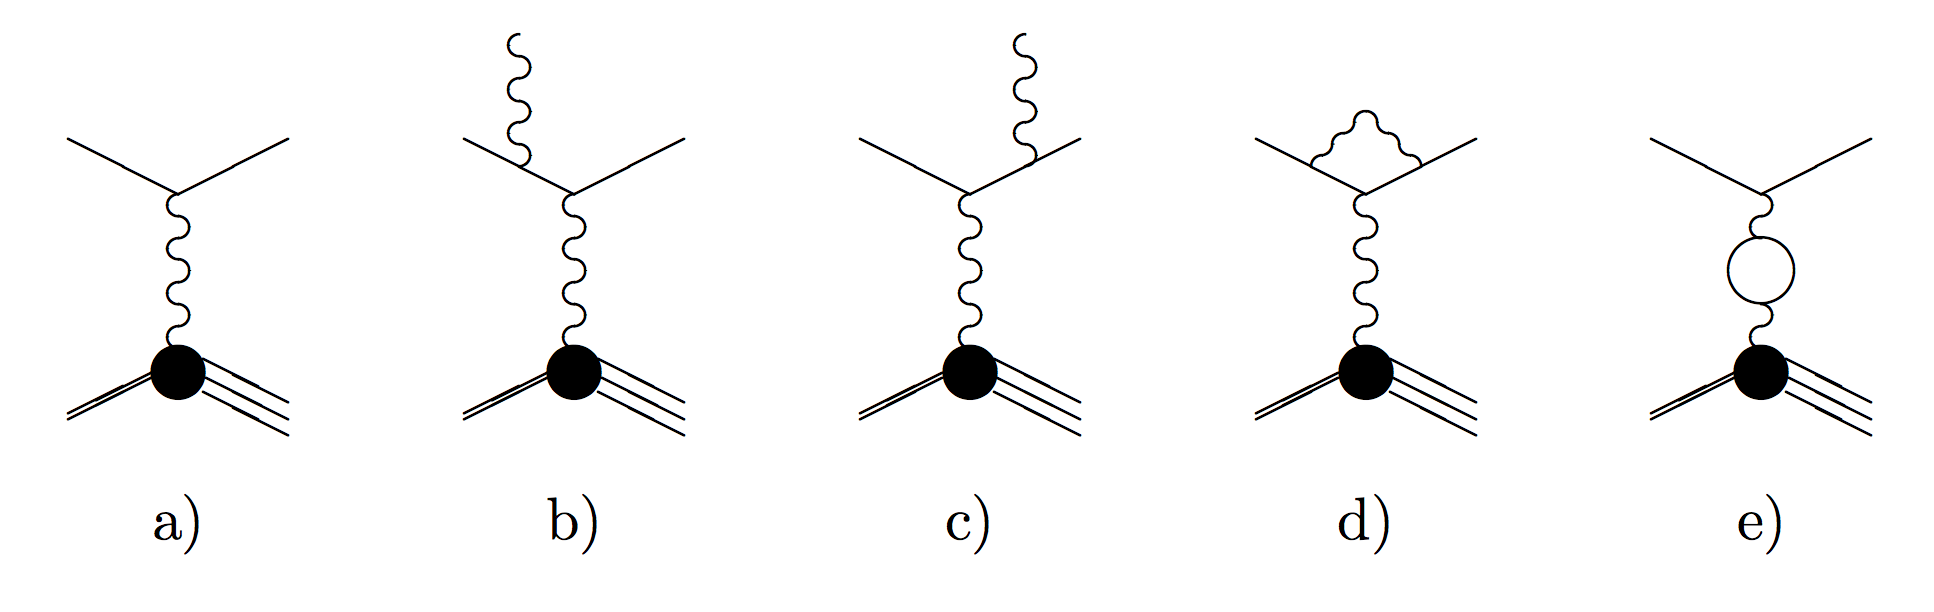
\epsfig{file=gfx/all_rad_feynm.png,width=12cm}}
\caption{List of the diagrams used for the calculation of the radiative corrections. From left to right, tree level, internal bremsstrahlung (incoming and outgoing leptons), vertex correction and vacuum polarization.}\label{fig:rad_dia}
\end{figure}

Correction to the quark line are not included in calculations, as explained in Section \ref{sec:RCF}. If we call $\sigma_{Born}$ the cross-section of the tree-level diagram and $\sigma_{Born+o(\alpha)}$ the cross-section of tree-level plus the first order correction enumerated above, the definition of the radiative corrections factor $\eta$ is :

\begin{equation} \label{eq:RCF_def}
  \eta(x,y)=\frac{\sigma_{Born}(x,y)}{\sigma_{Born+o(\alpha)}(x,y)}
\end{equation}

Obviously, the emission of a real photon is modifying the kinematic variables of the event. Let us take the case of one DIS event and a second one which is exactly like the first one except there is an ISR. The two events will share the same leptonic variables but they will have different hadronic variables. In the case of multiplicities, this discrepancy in the kinematic variables induces that some hadrons are falling into the wrong (x,y) bin. Applying the correction factor $\eta$ to the multiplicities is redirecting the hadrons to the right (x,y) bins.

\subsection{About emission of radiative photons}

There are two privileged angles (Fig. \ref{fig:plan}) for emission of a real photon :
\begin{itemize}
\item One in the direction of the incident lepton (s-peak)
\item One in the direction of the outgoing lepton (p-peak)
\end{itemize}

\begin{figure}[h!]
\centering
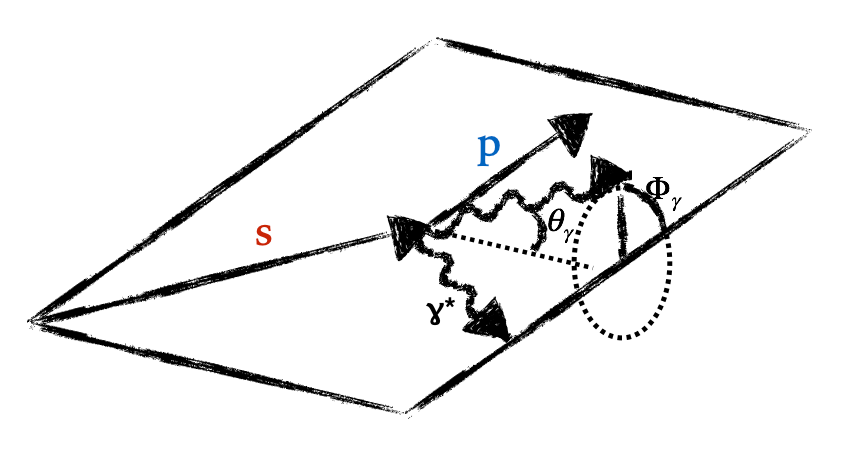
\includegraphics[width=12cm]{gfx/plan_angle.png}
\caption{Angles characterizing the emission of a radiative photon. The plane is defined by the incoming lepton (s) and the outgoing lepton (p). $\theta_\gamma$ is the polar angle and $\Phi_\gamma$ the azimuthal angle. The different $4$-momenta are : $s$ for incident lepton, $p$ for scattered lepton, $t$ for target proton, $k$ for real photon, $p_f$ for hadronic final state. Figure taken from \cite{TERAD2}.}
\label{fig:plan}
\end{figure}

In the case of muons, note that the $s$ and $p$ peaks are much less pronounced than for electrons.

This knowledge will later be useful to verify the consistency of DJANGOH results.

\subsection{About the radiative tail}

During elastic events, radiation of a real photon can still happen, modifying the leptonic variables of the events : this is the radiative tail. With Fig. \ref{fig:peaks}, we can see that even if we measure DIS events i.e. $Q^2$ $>$ 1, we still need informations on structure functions down to $Q^2$ = 0.

\begin{figure}[h!]
\centering
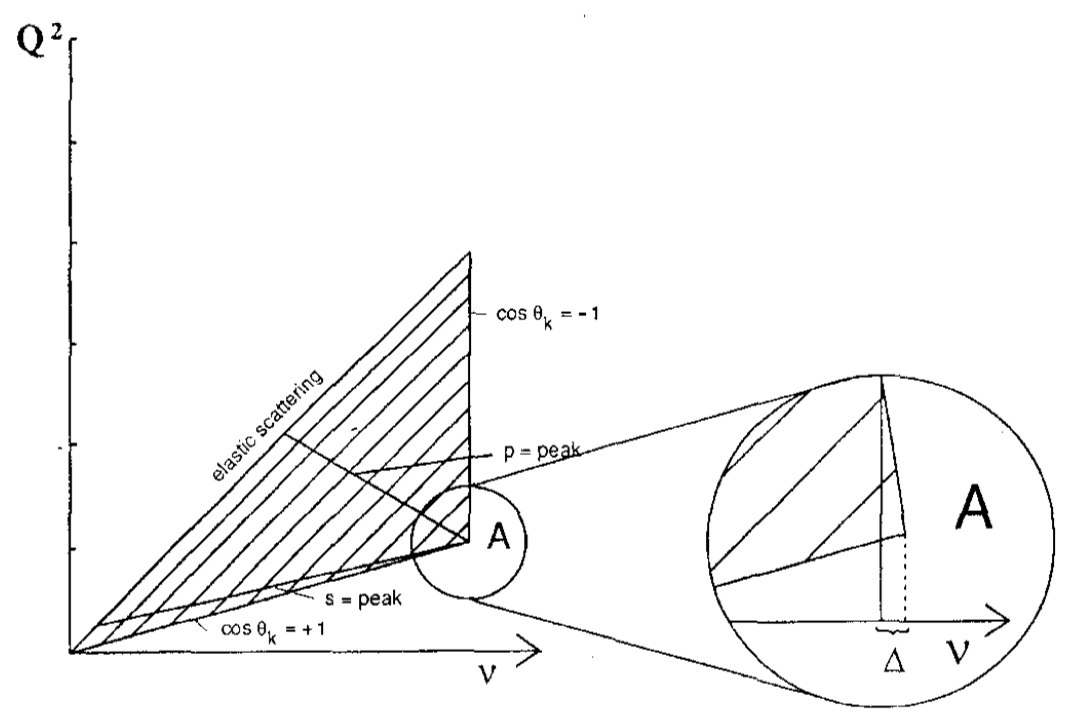
\includegraphics[width=12cm]{gfx/peaks.png}
\caption{Range of kinematical variables from which the radiative tails contribute to the cross section
measured at the point $A(Q^2, \nu)$. The s-peak is located near the boundary $cos\theta_\gamma=1$ which means
$\theta_\gamma \equiv 0[2\pi]$, thus collinear to the incoming lepton. The parallel lines are for constant $W$. Figure taken from \cite{TERAD2}.}
\label{fig:peaks}
\end{figure}

\newpage

%----------------------------------------------------------------------------------------

\section{Summary}

The renormalization is a necessary procedure when it comes to compute cross-sections as it allows to cure the divergences from the calculation and gives consistant results when compared to measurements. From this renormalization procedure arise radiative corrections which imply the emission of a real photon in the final state. These corrections can be splitted in three groups : from the Initial State Radiation (ISR), from the Final State Radiation (FSR) and from the Compton Peak. The emission of a real photon implies that there is a difference between the hadronic and leptonic variables that must be taken into account. Radiative correction factor are computed to measure the effect of the kinematic bin migration and correct the data accordingly.
